
%%%%%%%%%%%%%%%%%%%%%%%%%%%%%%%%%%%%%%%%%%%%%%%%%%%%%%%%%%%%%%%%%%%%%
%% This is a (brief) model paper using the achemso class
%% The document class accepts keyval options, which should include
%% the target journal and optionally the manuscript type.
%%%%%%%%%%%%%%%%%%%%%%%%%%%%%%%%%%%%%%%%%%%%%%%%%%%%%%%%%%%%%%%%%%%%%
\documentclass[journal=jpcb,manuscript=article]{achemso}

%%%%%%%%%%%%%%%%%%%%%%%%%%%%%%%%%%%%%%%%%%%%%%%%%%%%%%%%%%%%%%%%%%%%%
%% Place any additional packages needed here.  Only include packages
%% which are essential, to avoid problems later.
%%%%%%%%%%%%%%%%%%%%%%%%%%%%%%%%%%%%%%%%%%%%%%%%%%%%%%%%%%%%%%%%%%%%%
\usepackage{chemformula} % Formula subscripts using \ch{}
\usepackage[T1]{fontenc} % Use modern font encodings
%\usepackage{graphicx}
\usepackage{graphicx}
\usepackage{caption}
%%%%%%%%%%%%%%%%%%%%%%%%%%%%%%%%%%%%%%%%%%%%%%%%%%%%%%%%%%%%%%%%%%%%%
%% If issues arise when submitting your manuscript, you may want to
%% un-comment the next line.  This provides information on the
%% version of every file you have used.
%%%%%%%%%%%%%%%%%%%%%%%%%%%%%%%%%%%%%%%%%%%%%%%%%%%%%%%%%%%%%%%%%%%%%
%%\listfiles

%%%%%%%%%%%%%%%%%%%%%%%%%%%%%%%%%%%%%%%%%%%%%%%%%%%%%%%%%%%%%%%%%%%%%
%% Place any additional macros here.  Please use \newcommand* where
%% possible, and avoid layout-changing macros (which are not used
%% when typesetting).
%%%%%%%%%%%%%%%%%%%%%%%%%%%%%%%%%%%%%%%%%%%%%%%%%%%%%%%%%%%%%%%%%%%%%
\newcommand*\mycommand[1]{\texttt{\emph{#1}}}

%%%%%%%%%%%%%%%%%%%%%%%%%%%%%%%%%%%%%%%%%%%%%%%%%%%%%%%%%%%%%%%%%%%%%
%% Meta-data block
%% ---------------
%% Each author should be given as a separate \author command.
%%
%% Corresponding authors should have an e-mail given after the author
%% name as an \email command. Phone and fax numbers can be given
%% using \phone and \fax, respectively; this information is optional.
%%
%% The affiliation of authors is given after the authors; each
%% \affiliation command applies to all preceding authors not already
%% assigned an affiliation.
%%
%% The affiliation takes an option argument for the short name.  This
%% will typically be something like "University of Somewhere".
%%
%% The \altaffiliation macro should be used for new address, etc.
%% On the other hand, \alsoaffiliation is used on a per author basis
%% when authors are associated with multiple institutions.
%%%%%%%%%%%%%%%%%%%%%%%%%%%%%%%%%%%%%%%%%%%%%%%%%%%%%%%%%%%%%%%%%%%%%
\author{Sree ganesh balasubramani}
\affiliation{Department of Chemistry and Biochemistry, University of Arizona, Tucson, Arizona 85721, United States}
\author{Steven D. Schwartz}
\affiliation{Department of Chemistry and Biochemistry, University of Arizona, Tucson, Arizona 85721, United States}
%\author{I. Ken Groupleader}
%\altaffiliation{A shared footnote}
\email{sschwartz@email.arizona.edu}
%\phone{+123 (0)123 4445556}
%\fax{+123 (0)123 4445557}
%\affiliation[Unknown University]
%{Department of Chemistry, Unknown University, Unknown Town}
%\alsoaffiliation[Second University]
%{Department of Chemistry, Second University, Nearby Town}

%%%%%%%%%%%%%%%%%%%%%%%%%%%%%%%%%%%%%%%%%%%%%%%%%%%%%%%%%%%%%%%%%%%%%
%% The document title should be given as usual. Some journals require
%% a running title from the author: this should be supplied as an
%% optional argument to \title.
%%%%%%%%%%%%%%%%%%%%%%%%%%%%%%%%%%%%%%%%%%%%%%%%%%%%%%%%%%%%%%%%%%%%%
\title[]
  {Transition path sampling and the calculation of free energies of enzymatic
  reactions}
%%%%%%%%%%%%%%%%%%%%%%%%%%%%%%%%%%%%%%%%%%%%%%%%%%%%%%%%%%%%%%%%%%%%%
%% Some journals require a list of abbreviations or keywords to be
%% supplied. These should be set up here, and will be printed after
%% the title and author information, if needed.
%%%%%%%%%%%%%%%%%%%%%%%%%%%%%%%%%%%%%%%%%%%%%%%%%%%%%%%%%%%%%%%%%%%%%
\abbreviations{TPS,NMR,UV}
\keywords{American Chemical Society, \LaTeX}

%%%%%%%%%%%%%%%%%%%%%%%%%%%%%%%%%%%%%%%%%%%%%%%%%%%%%%%%%%%%%%%%%%%%%
%% The manuscript does not need to include \maketitle, which is
%% executed automatically.
%%%%%%%%%%%%%%%%%%%%%%%%%%%%%%%%%%%%%%%%%%%%%%%%%%%%%%%%%%%%%%%%%%%%%
\begin{document}

%%%%%%%%%%%%%%%%%%%%%%%%%%%%%%%%%%%%%%%%%%%%%%%%%%%%%%%%%%%%%%%%%%%%%
%% The "tocentry" environment can be used to create an entry for the
%% graphical table of contents. It is given here as some journals
%% require that it is printed as part of the abstract page. It will
%% be automatically moved as appropriate.
%%%%%%%%%%%%%%%%%%%%%%%%%%%%%%%%%%%%%%%%%%%%%%%%%%%%%%%%%%%%%%%%%%%%%
%\begin{tocentry}

%Some journals require a graphical entry for the Table of Contents.
%This should be laid out ``print ready'' so that the sizing of the
%text is correct.

%Inside the \texttt{tocentry} environment, the font used is Helvetica
%8\,pt, as required by \emph{Journal of the American Chemical
%Society}.

%The surrounding frame is 9\,cm by 3.5\,cm, which is the maximum
%permitted for  \emph{Journal of the American Chemical Society}
%graphical table of content entries. The box will not resize if the
%content is too big: instead it will overflow the edge of the box.

%This box and the associated title will always be printed on a
%separate page at the end of the document.

%\end{tocentry}

%%%%%%%%%%%%%%%%%%%%%%%%%%%%%%%%%%%%%%%%%%%%%%%%%%%%%%%%%%%%%%%%%%%%%
%% The abstract environment will automatically gobble the contents
%% if an abstract is not used by the target journal.
%%%%%%%%%%%%%%%%%%%%%%%%%%%%%%%%%%%%%%%%%%%%%%%%%%%%%%%%%%%%%%%%%%%%%
\begin{abstract}
  We discuss a scheme for the calculation of free energies within 
  the transition path sampling (TPS) method. TPS is often used for
  the calculations of reaction coordinates of complex reactions in 
  the condensed phase and in this work we use it to sample the 
  equilibrium distribution of the reaction coordinate. This 
  distribution can then be used for the calculations of free energies
  using standard Boltzmann inversion schemes. We calculate the free
  energy profiles of the human Mat2a enzyme and the plasmodium 
  adenosine deaminase to demonstrate the applicability of this method
  for enzyme catalysis reactions. 

  %This is an example document for the \textsf{achemso} document
  %class, intended for submissions to the American Chemical Society
  %for publication. The class is based on the standard \LaTeXe\
  %\textsf{report} file, and does not seek to reproduce the appearance
  %of a published paper.

  %This is an abstract for the \textsf{achemso} document class
  %demonstration document.  An abstract is only allowed for certain
  %manuscript types.  The selection of \texttt{journal} and
  %\texttt{manuscript} will determine if an abstract is valid.  If
  %not, the class will issue an appropriate error.
\end{abstract}

%%%%%%%%%%%%%%%%%%%%%%%%%%%%%%%%%%%%%%%%%%%%%%%%%%%%%%%%%%%%%%%%%%%%%
%% Start the main part of the manuscript here.
%%%%%%%%%%%%%%%%%%%%%%%%%%%%%%%%%%%%%%%%%%%%%%%%%%%%%%%%%%%%%%%%%%%%%
\section{Introduction}
Atomistic level study of the mechanism of enzyme catalysis is necessary
to understand the efficiency of enzymes as well as to device strategies for inhibiting 
their activity. 
Transition path sampling \cite{Bolhuis02AnnRevPhysChem53p291,Dellago98JChemPhys108p1964}
Human Mat2a enzyme and plasmodium vivax adenosine deaminase \cite{Luo07JAmChemSoc129p8008} 
\section{Theory}
\subsection{Transition path sampling}
%Transition path sampling is an importance sampling in the trajectory space.
Consider the molecular dynamics simulation of a molecular system consisting 
of $N$ atoms. Starting from the initial positions and momenta of each atom at time $t_0$,
the time evolution is carried out by finding the position ($\textbf{q}$) and 
momenta ($\textbf{p}$) of each atom at regular intervals of time $t_i = t_0 + i\Delta t$  
($i = 0,1,2,\ldots$). At each of the time slices, the positions and momenta can be collectively represented as
the set $z = \{\textbf{q},\textbf{p}\}$. If the MD simulation is run for a total 
time of $\mathcal{T}$ the number of time slices is given by $L = \mathcal{T}/\Delta t +1$ and for this sequence of 
times the state of the system can be represented as 
\begin{equation}
z(\mathcal{T}) = \{z_0, z_{\Delta t}, z_{2\Delta t},\ldots,z_{\mathcal{T}}\}
\end{equation}
The probability to obtain a particular sequence of states is determined by the initial 
conditions and the type of dynamics used for the time evolution. If the time evolution is 
Markovian, the probability to go from $z_{i\Delta t}$ to $z_{(i+1)\Delta t}$ depends only 
on $z_{i\Delta t}$ and not on conditions before the time $i\Delta t$ the total path probablility can 
be expressed as the product of individual probabilities $p(i\rightarrow j)$ as 
\begin{equation}
\mathcal{P}[z(\mathcal{T})] = \rho(z_0)\Pi_{i=0}^{\mathcal{T}/\Delta t-1} p(z_{i\Delta t}\rightarrow z_{(i+1)\Delta t}),
\end{equation}
where $\rho(z_0)$ is the equilibrium distribution of the initial conditions and for a canonical ensemble this can be 
expressed as 
\begin{equation}
\rho(z_0) = \exp(-\beta H(z_0))/Z
\end{equation}
where 
\begin{equation}
Z = \int dz \exp(-\beta H(z)) 
\end{equation}
is the canonical partition function. 

Within the transition path sampling, the trajectories of interest start in the reactant region of the 
phase space ($\mathcal{A}$) and end in the product region ($\mathcal{B}$). Such reactive trajectories have 
a restricted probability distribution function given by
\begin{equation}
\mathcal{P}_{\mathcal{AB}}[z_{\mathcal{T}}] = h_{\mathcal{A}}(z_0)\mathcal{P}[z(\mathcal{T})]
h_{\mathcal{B}}(z_{\mathcal{T}})/Z_{\mathcal{AB}}(\mathcal{T})\label{eqn:tpsensem}
\end{equation}
where 
\[
    h_{\mathcal{A}/\mathcal{B}}(z)= 
\begin{cases}
    1, & \text{if } z\in \mathcal{A}/\mathcal{B}\\
    0,              & \text{otherwise}
\end{cases}
\]
The set of all reactive trajectories characterized by the distribution function
given by Eq. \ref{eqn:tpsensem} is the transition path ensemble. 

\subsection{Equilibrium distribution of order parameters}
%Monte carlo methods in trajectory space the probability of a path is 
%\begin{equation}
%P(x_A)
%\end{equation}
The free energy as a function of the order parameter $\zeta$ is defined
as 
\begin{equation}
\text{A}(\zeta) = -k_{\text{B}}T\text{ln}(P(\zeta)) + C, \label{eqn:fenergy}
\end{equation}
where $P(\zeta)$ is the probability distribution of the reaction coordinate
$\zeta$ and $C$ is an arbitrary constant. At equilibrium the probability distribution of the 
reaction coordinate 
can be obtained from the distribution function for the phase space $\rho(\textbf{q})$ as
\begin{equation}
P(\zeta) = \int d\textbf{V} \rho(\textbf{q})\delta\left[\zeta-\tilde{\zeta}(\textbf{q})\right].
\end{equation}
The integration is over the entire phase space. In practice the calculation of this distribution function
often proceeds using histogram based methods where the reaction coordinate is 
divided into bins and the frequency of the occurence of the reaction coordinate within a particular window
during the course of molecular dynamics simulations is used to calculate the probability distribution. 
Since some values of the reaction coordinates particulary close to the transition state are 
rarely sampled in a conventional MD simulations, enhanced sampling techniques such as the umbrella sampling
are necessary to sample the low probability regions. TPS is designed to sample these regions in phase space 
without the application of any external bias, but the trajectories sampled with TPS are only reactive and hence
they are not distributed according to the equilibrium distribution function. 
The restriction that the pathways start from the reactant state and end in the product state can be relaxed
to obtain an ensemble of trajectories that will be distributed according to the equilibrium distribution. 

\subsection{The algorithm}
We follow the steps proposed by Radhakrishnan et al. \cite{Radhakrishnan04JChemPhys121p2436} 
to sample TPS trajectories within windows of the order parameter. 
\begin{itemize}
  \item An appropriate order parameter is chosen for the reaction of interest 
  that can distinguish the reactant and product states sufficiently well and the TPS ensemble is harvested 
  which consists only of reactive trajectories.
\item Divide the order parameter into windows $\{\zeta_i\}$ within which the 
order parameters are given by 
$\zeta_{i}^{min} < \zeta < \zeta_{i}^{max}$.
\item Choose a reactive trajectory $\tilde{z}(\mathcal{T})$ from the TPS ensemble as 
a guiding trajectory for the window sampling. Pick a time slice from this trajectory 
$\tilde{z}_{j\Delta t}$ such that the order parameter calculated for this time slice
$\tilde{\zeta}$ satisfies $\zeta_{i}^{min} < \tilde{\zeta} < \zeta_{i}^{max}$.
\item Using the shooting and shifting algorithm familiar from TPS simulations, harvest 
dynamics trajectories starting from the time slice $\tilde{z}_{j\Delta t}$ of the trajectory 
  $\tilde{z}(\mathcal{T})$ and accept the new trajectory if at any time slice the calculated 
  order parameter $\hat{\zeta}$ satisfies $\zeta_{i}^{min} < \hat{\zeta} < \zeta_{i}^{max}$.
  \item Calculate the probability distribution ($P_i(\zeta)$) within the window $\zeta_{i}^{min} 
  < \zeta < \zeta_{i}^{max}$ by constructing histograms obtained from the ensemble of 
  accepted trajectories for the window $i$. 
  \item Combine the probability distributions in successive windows by adjusting the constants $C$
  such that the free energy $A$ from Eq. \ref{eqn:fenergy} is continuous. 
\end{itemize}   

\section{Results and discussion}
%\begin{figure}
%\centering
%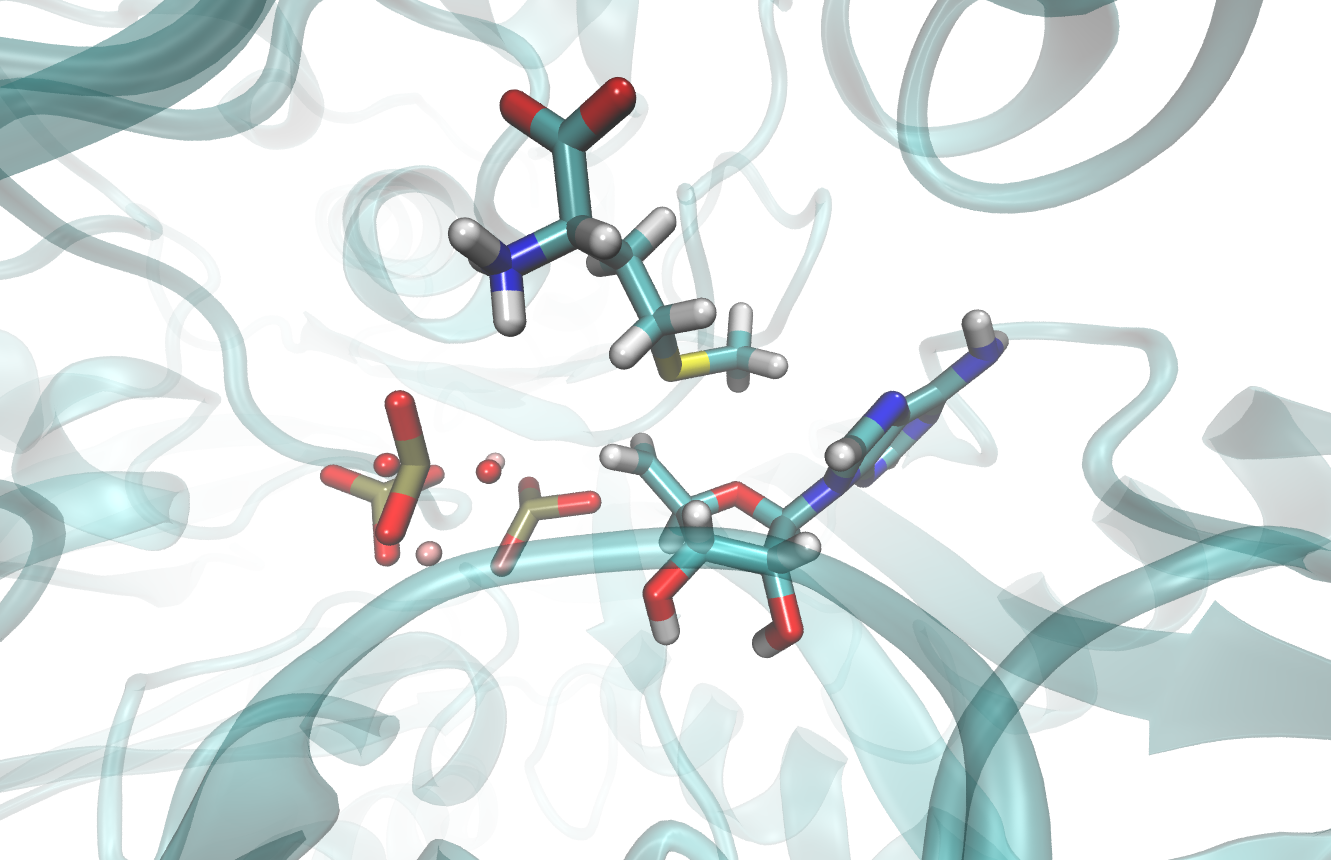
\includegraphics[scale=0.2 ]{figures/ts253.png}
%\caption{Enzymatic reaction in human Mat2a enzyme}
%  \label{fgr:mat2a_reaction}
%\end{figure}
\section{Adenosine deaminase reaction coordinates and free energy}
\begin{figure}[ht]
\centering
\begin{minipage}[b]{0.32\linewidth}
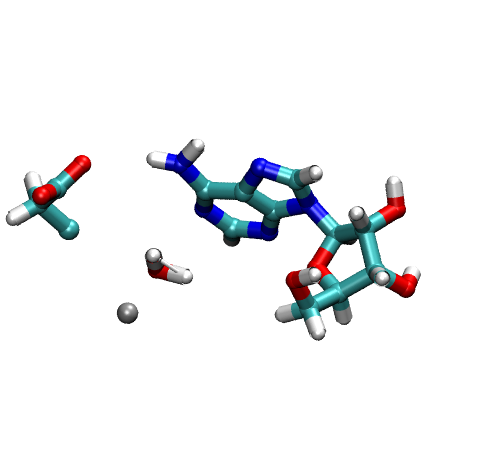
\includegraphics[scale=0.3]{figures/reactant-state.png}
\caption{Reactant state}
\label{fig:minipage1}
\end{minipage}
\quad
\begin{minipage}[b]{0.32\linewidth}
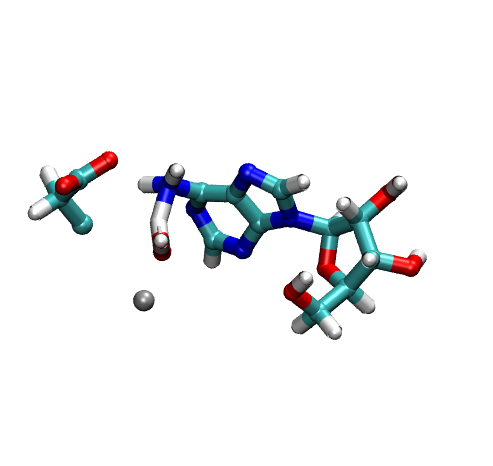
\includegraphics[scale=0.3]{figures/int1.png}
\caption{Intermediate state}
\label{fig:minipage2}
\end{minipage}
\quad
\begin{minipage}[b]{0.32\linewidth}
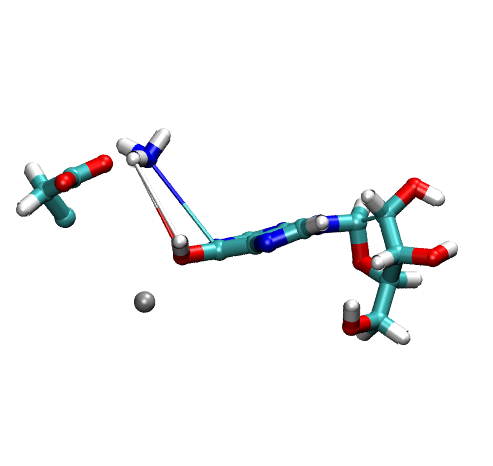
\includegraphics[scale=0.3]{figures/product-state.png}
\caption{Product state}
\label{fig:minipage1}
\end{minipage}
\end{figure}

%\subsection{Outline}
\begin{figure}[ht]
\centering
\begin{minipage}[b]{0.45\linewidth}
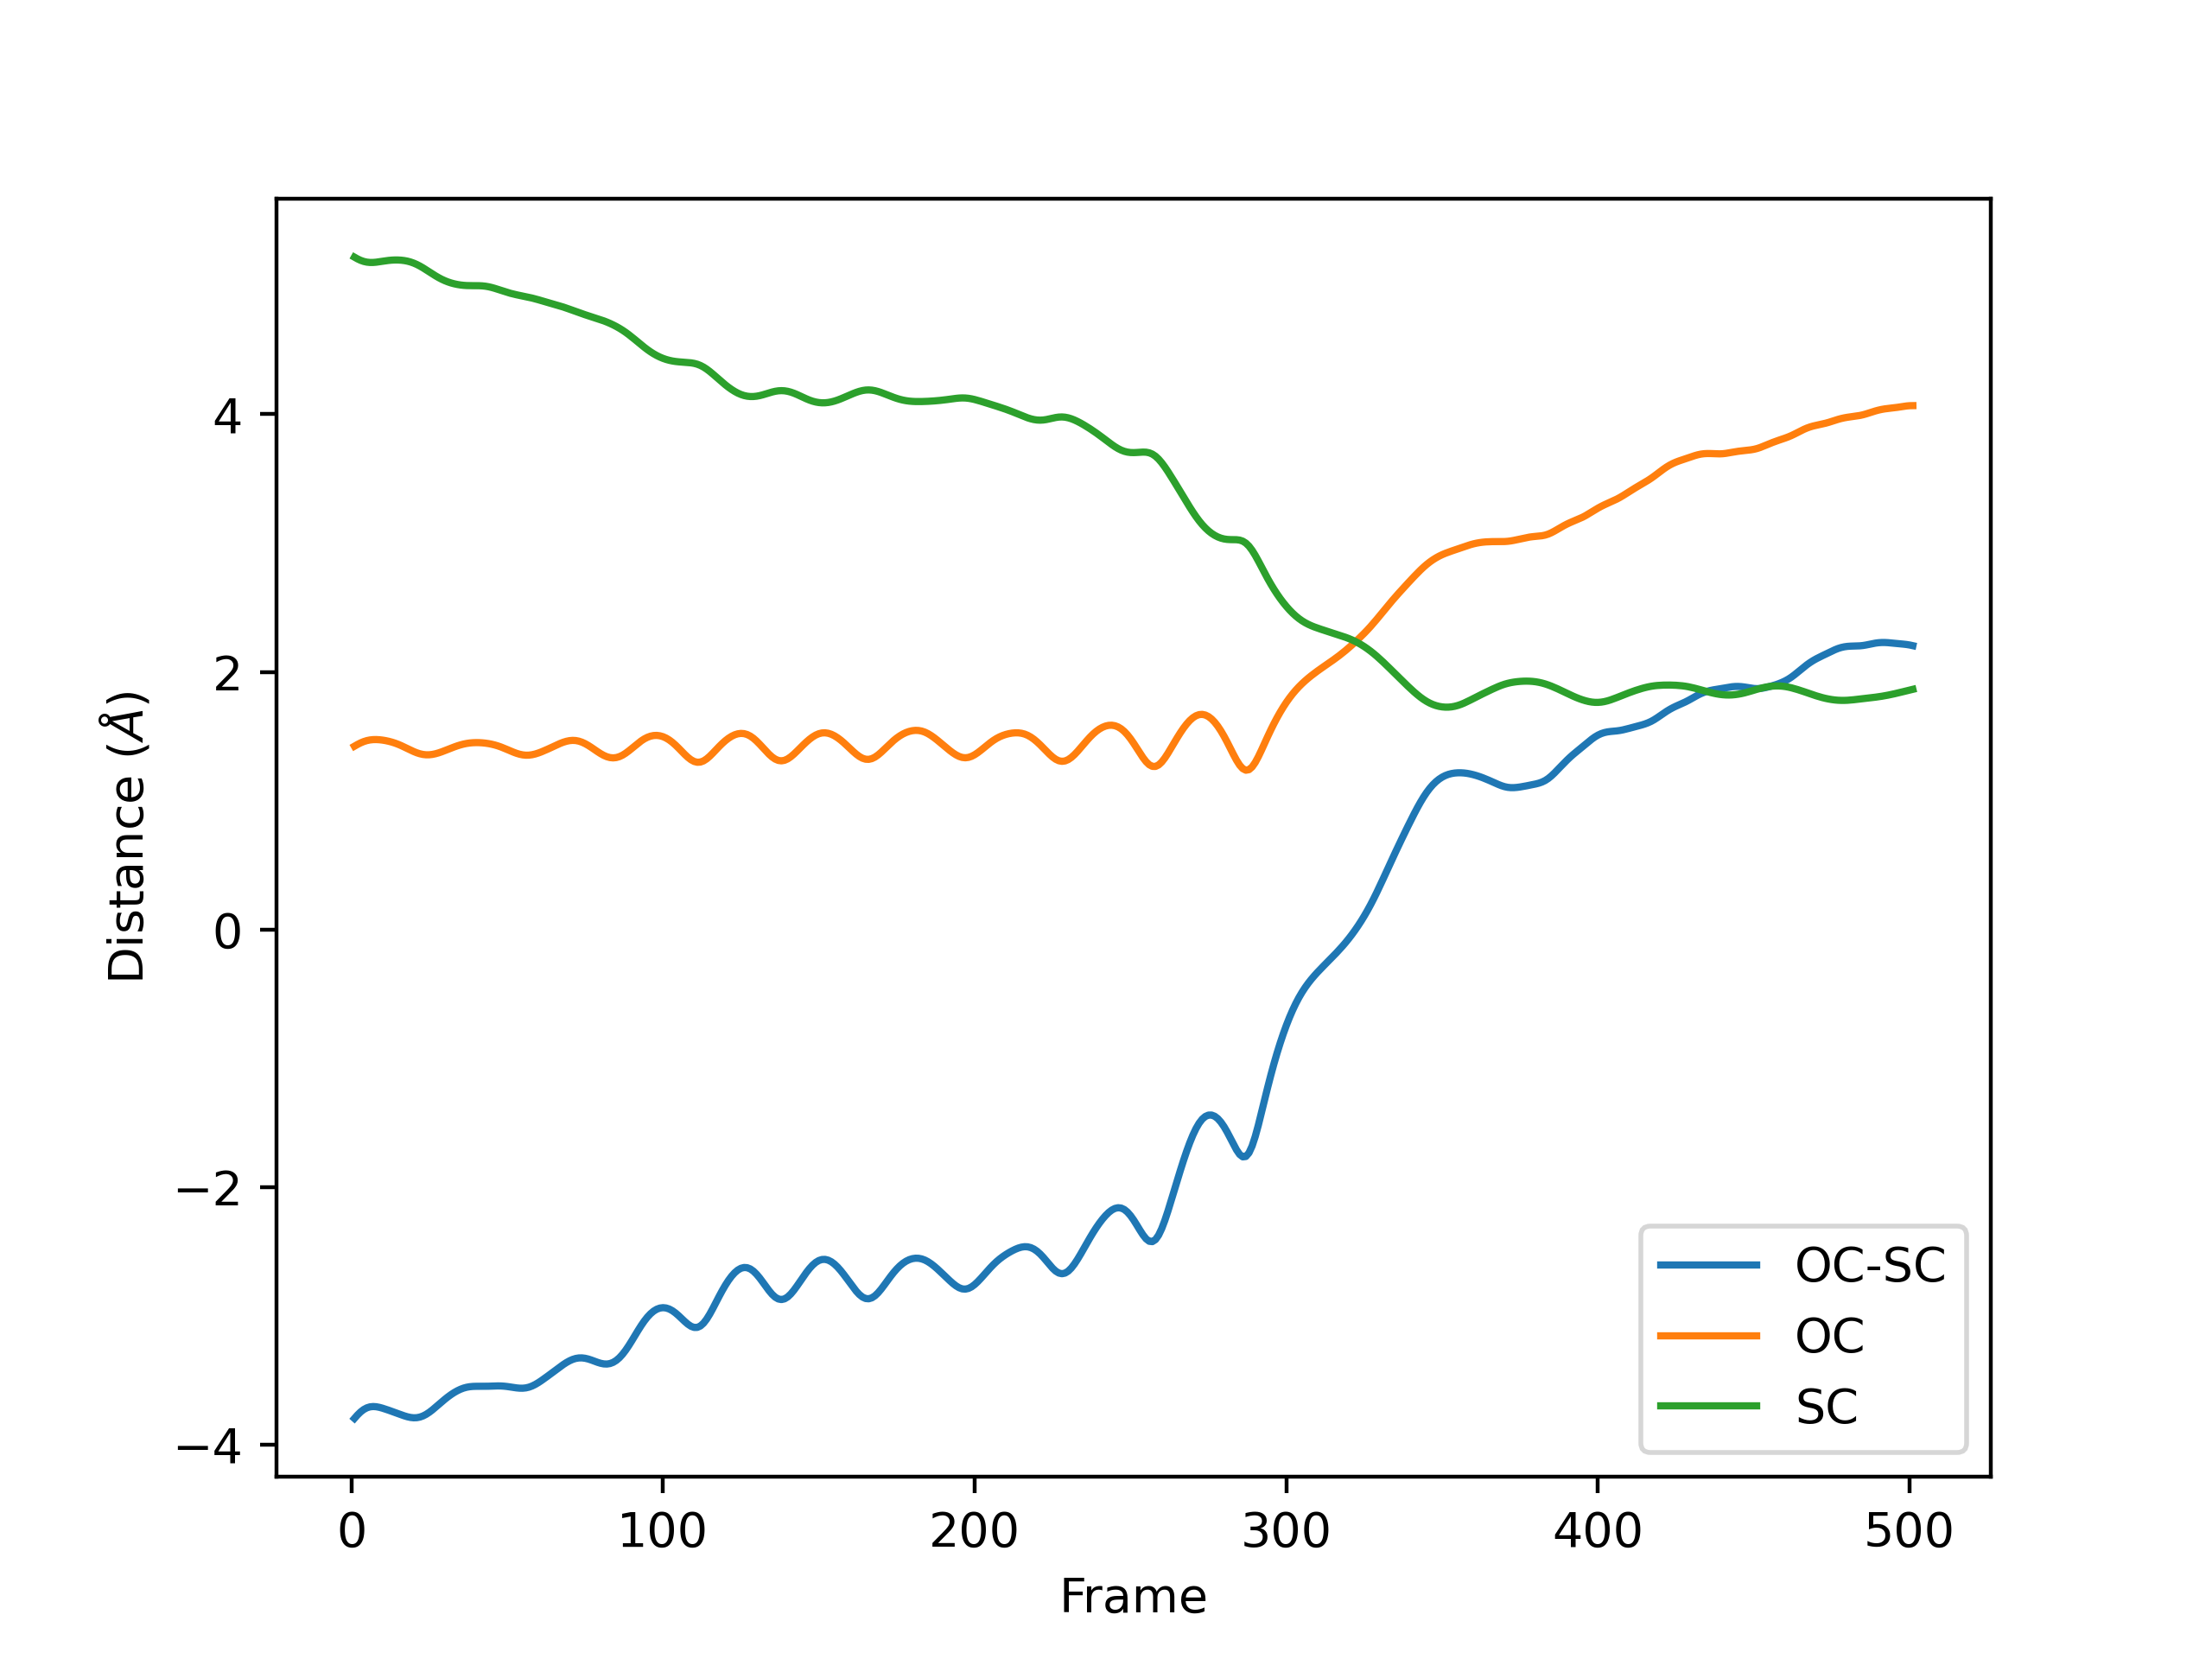
\includegraphics[scale=0.5]{figures/reac-sc-oc-167.png}
\caption{Trajectory 167}
\label{fig:minipage1}
\end{minipage}
\quad
\begin{minipage}[b]{0.45\linewidth}
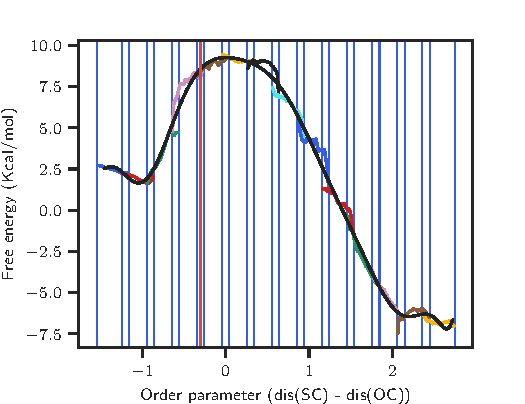
\includegraphics[scale=0.9]{figures/den-fenergy-1.pdf}
\caption{Free energy profile for the enzymatic reaction in human Mat2a enzyme}
\label{fig:minipage2}
\end{minipage}
\end{figure}

%%%%%%%%%%%%%%%%%%%%%%%%%%%%%%%%%%%%%%%%%%%%%%%%%%%%%%%%%%%%%%%%%%%%%
%% The "Acknowledgement" section can be given in all manuscript
%% classes.  This should be given within the "acknowledgement"
%% environment, which will make the correct section or running title.
%%%%%%%%%%%%%%%%%%%%%%%%%%%%%%%%%%%%%%%%%%%%%%%%%%%%%%%%%%%%%%%%%%%%%
\begin{acknowledgement}


\end{acknowledgement}

%%%%%%%%%%%%%%%%%%%%%%%%%%%%%%%%%%%%%%%%%%%%%%%%%%%%%%%%%%%%%%%%%%%%%
%% The same is true for Supporting Information, which should use the
%% suppinfo environment.
%%%%%%%%%%%%%%%%%%%%%%%%%%%%%%%%%%%%%%%%%%%%%%%%%%%%%%%%%%%%%%%%%%%%%
\begin{suppinfo}


\end{suppinfo}

%%%%%%%%%%%%%%%%%%%%%%%%%%%%%%%%%%%%%%%%%%%%%%%%%%%%%%%%%%%%%%%%%%%%%
%% The appropriate \bibliography command should be placed here.
%% Notice that the class file automatically sets \bibliographystyle
%% and also names the section correctly.
%%%%%%%%%%%%%%%%%%%%%%%%%%%%%%%%%%%%%%%%%%%%%%%%%%%%%%%%%%%%%%%%%%%%%
\bibliography{manuscript}

\end{document}
